\label{sec:impacts_SR3P_inclusive}

\begin{figure}
  \centering
  \includegraphics[height=0.33\textheight]{Figures/dataMC/Run2/phoCR/SR3P/SYS_mWZGloose_central_pow\dataMCblind .pdf}
  \hfill
  \includegraphics[height=0.33\textheight]{Figures/combine/inclusive/impacts_\expobs_Run2_SR3P_phoCR_lepMC_mWZGloose.pdf}
  \caption{\captionImpact{transverse mass of the $\PW\PZ\PGg$ system}{Loose}{cut-based ID}{d}{not }}
  \label{fig:inclusive_cutID_phoCR_mWZGloose}
\end{figure}

\begin{figure}
  \centering
  \includegraphics[height=0.33\textheight]{Figures/dataMC/Run2/fullMC/SR3P/SYS_mWZGloose_central_pow\dataMCblind .pdf}
  \hfill
  \includegraphics[height=0.33\textheight]{Figures/combine/inclusive/impacts_\expobs_Run2_SR3P_phoMC_lepMC_mWZGloose.pdf}
  \caption{\captionImpact{transverse mass of the $\PW\PZ\PGg$ system}{Loose}{cut-based ID}{s}{not }}
  \label{fig:inclusive_cutID_phoMC_mWZGloose}
\end{figure}

The largest systematic uncertainty is the QCD scale, which accounts for a shift of
$\approx \pm 0.3$ on the signal strength $\mu$.
\note{I checked, and it is NOT applied to the signal, like I did in June last year for 4L (Gullielmo's comment).
  On $\PW\PZ$ it has a $\approx 15\usep\%$ effect (Fig.~\ref{fig:debug_SR3P_WZTo3LNu_QCDScale}).
  $\PZ\PGg$ has also a $\approx 18\usep\%$ effect (Fig~\ref{fig:debug_SR3P_ZGToLLG_QCDScale}).
  }
The leading experimental uncertainty is due to the electron efficiency scale factors,
similarly to the four lepton channel.

% <DEBUG>
\begin{figure}
  \centering
  \subfigure [] {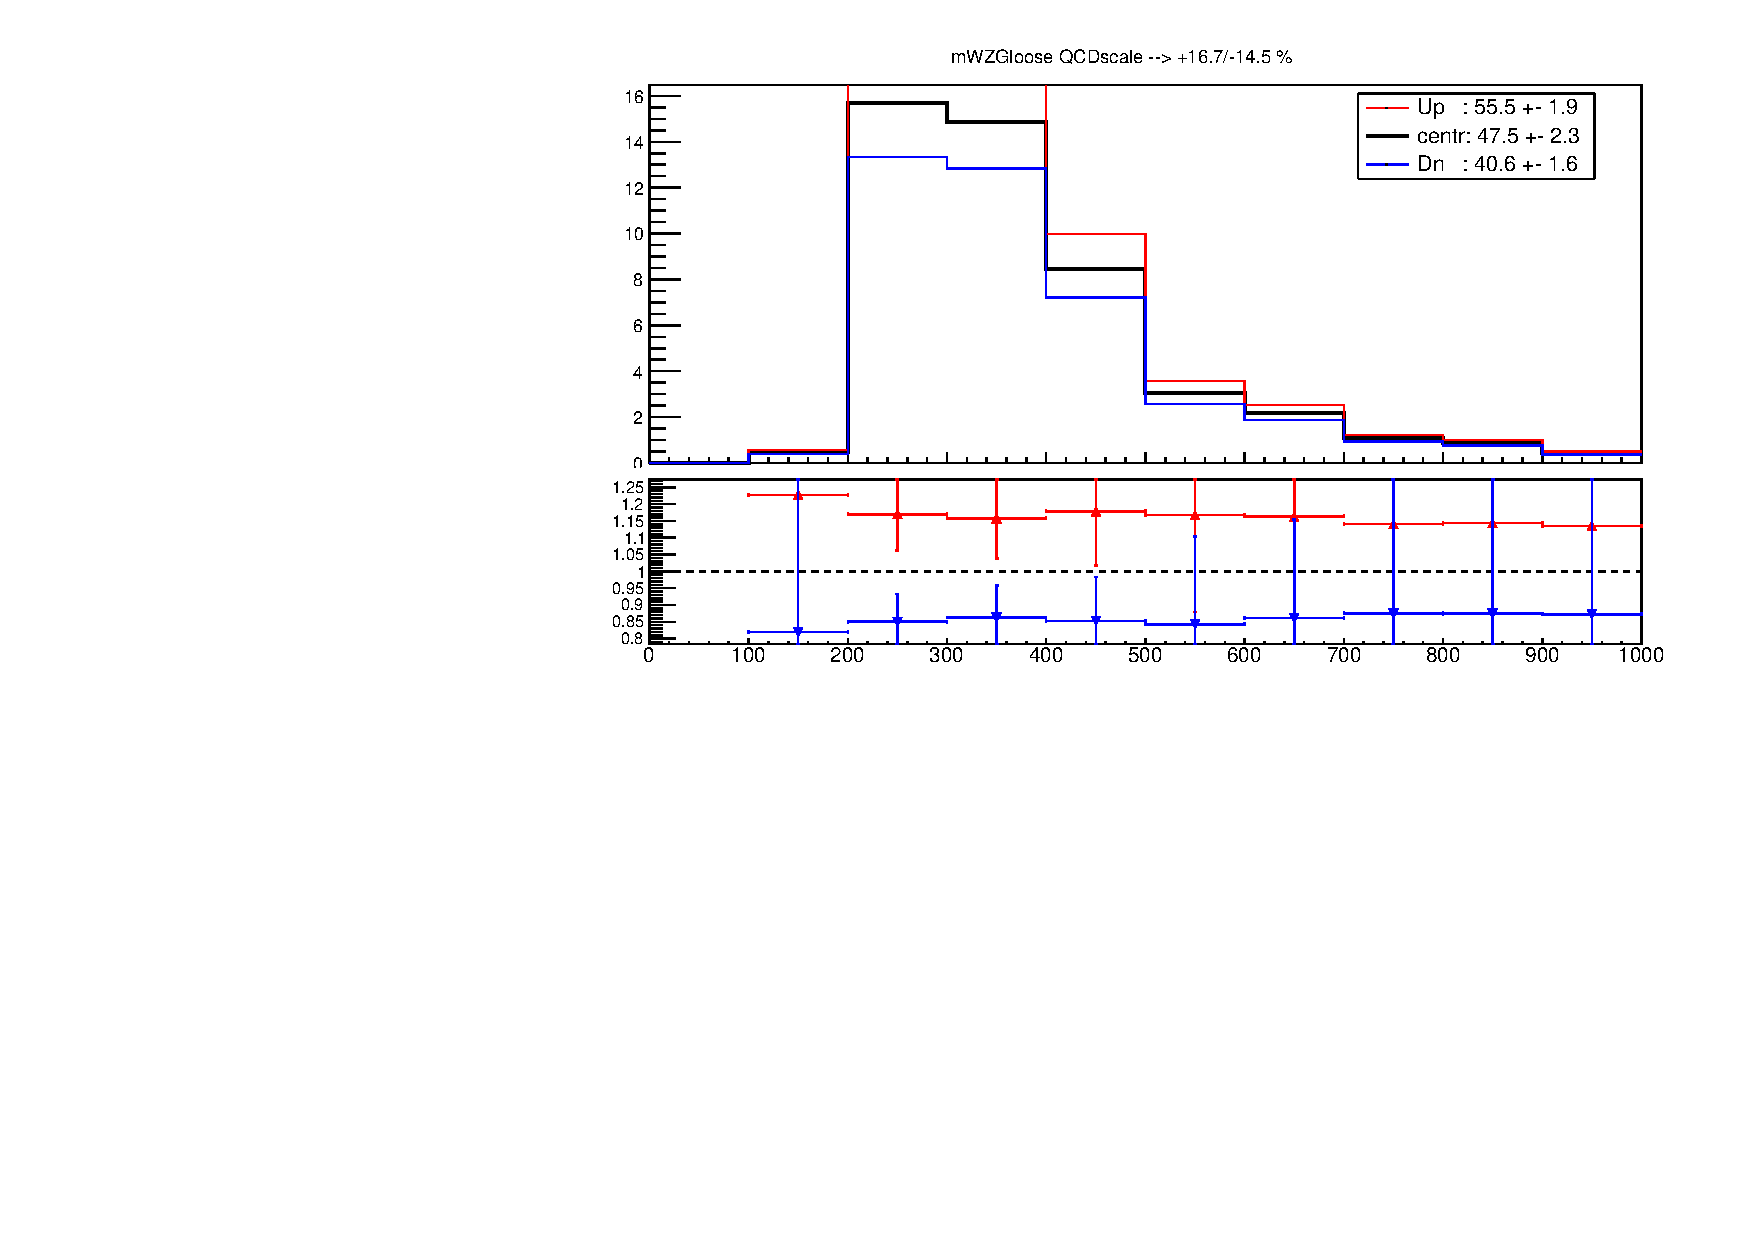
\includegraphics[width=.495\textwidth]{Figures/SYS/SR3P/WZTo3LNu_mWZGloose_QCDscale.pdf}\label{fig:debug_SR3P_WZTo3LNu_QCDScale}}
  \subfigure [] {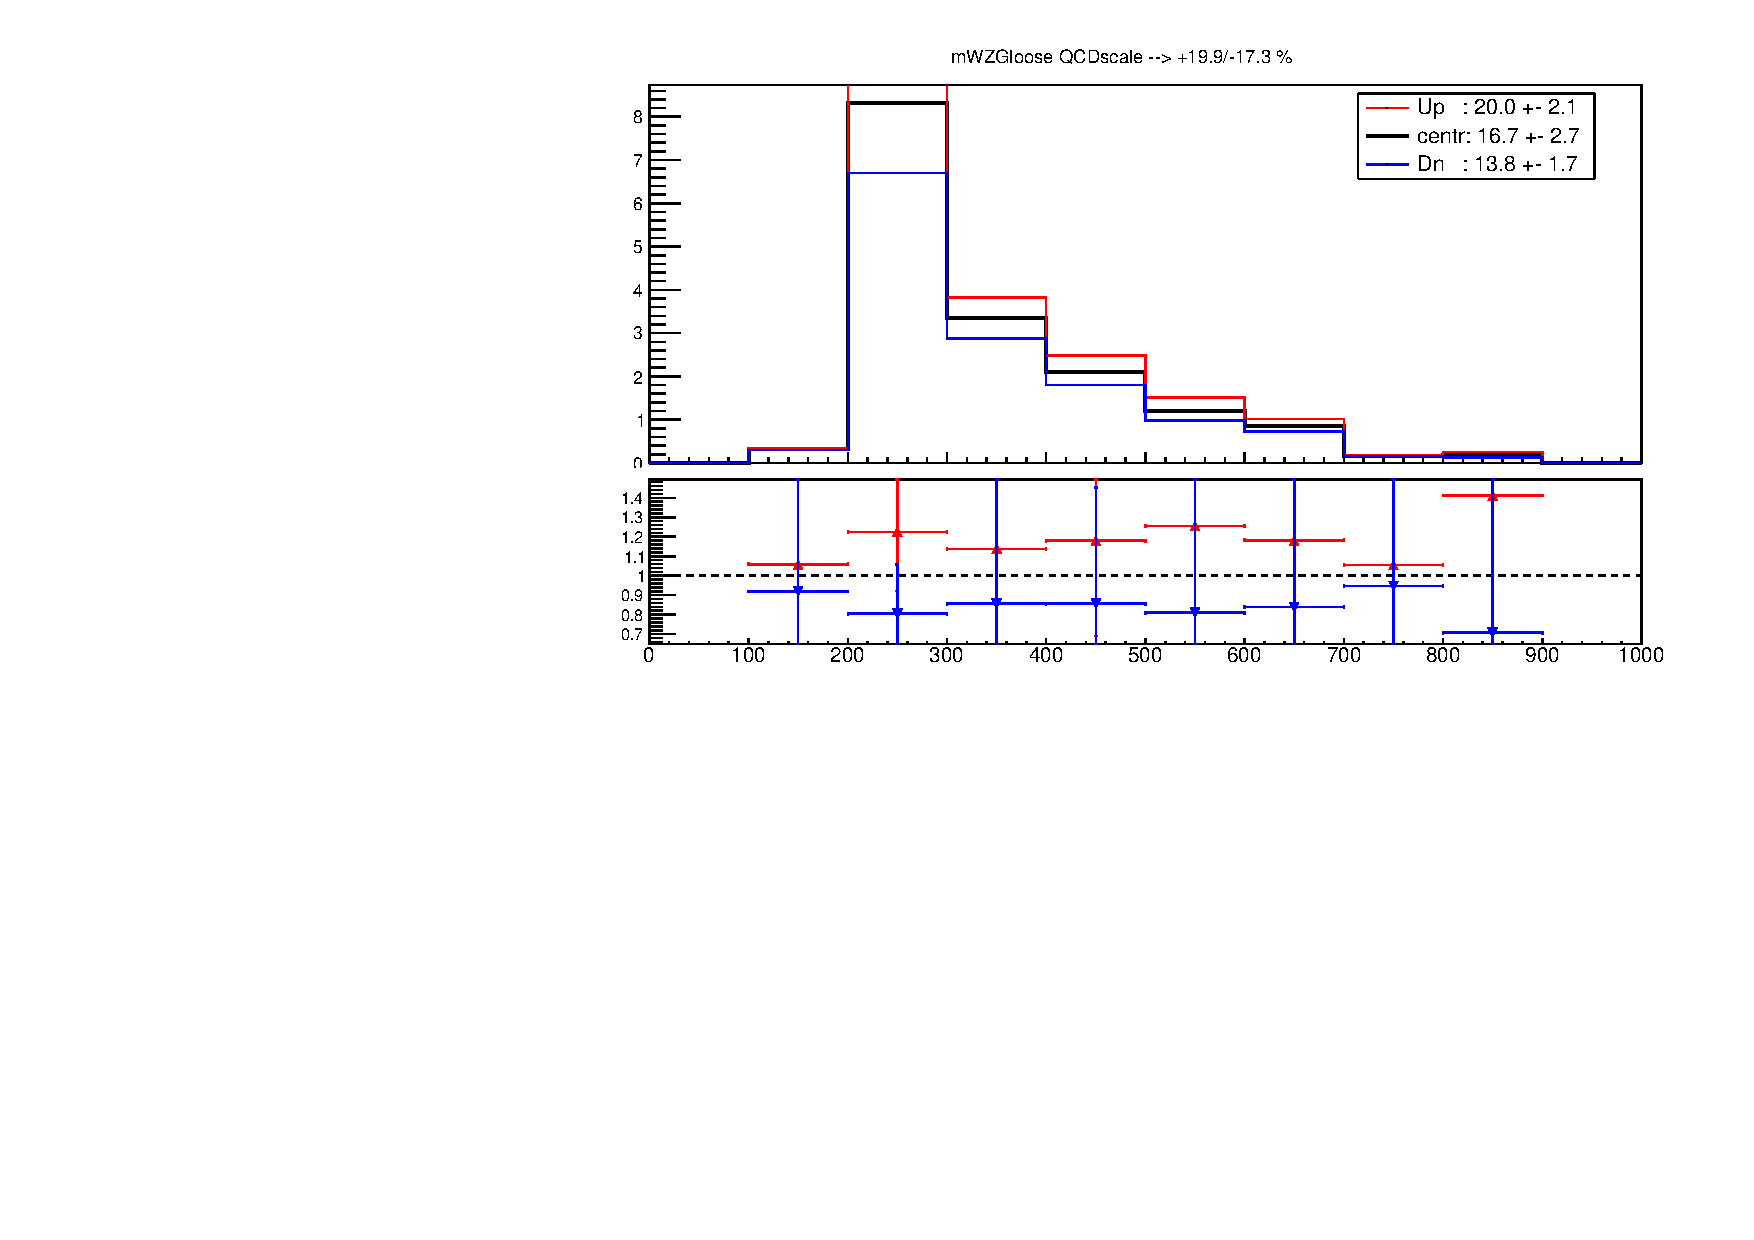
\includegraphics[width=.495\textwidth]{Figures/SYS/SR3P/ZGToLLG_mWZGloose_QCDscale.pdf}\label{fig:debug_SR3P_ZGToLLG_QCDScale}}
  \caption{\note{}: Effect of the QCD scale systematic on $\PW\PZ$ (left) and $\PZ\PGg$ in SR3P ($m_{\PW\PZ\PGg}$)}
\end{figure}
% </DEBUG>
